\section{Harness}
\label{sec:harness}

\subsection{System and task context}

The harness combines Astra's task reasoning and supervision with VLA execution and direct intervention (Figure~\ref{fig:architecture}). The system uses the official RoboMME GroundSG checkpoint for low-level control, while Astra selects subgoals, supervises execution, and intervenes directly when needed.

Before each Astra review, the VLA predicts an action sequence from the current observations and subgoal. The harness uses forward kinematics to estimate the corresponding end-effector motion, making the predicted actions easier for Astra to interpret. Astra then receives the task instruction, current front and wrist RGB images, robot state, and a summary of the VLA's predicted motion. It can also query archived observations and consult episode notes and relevant experience before making its next decision.

\begin{figure}[!htbp]
\centering
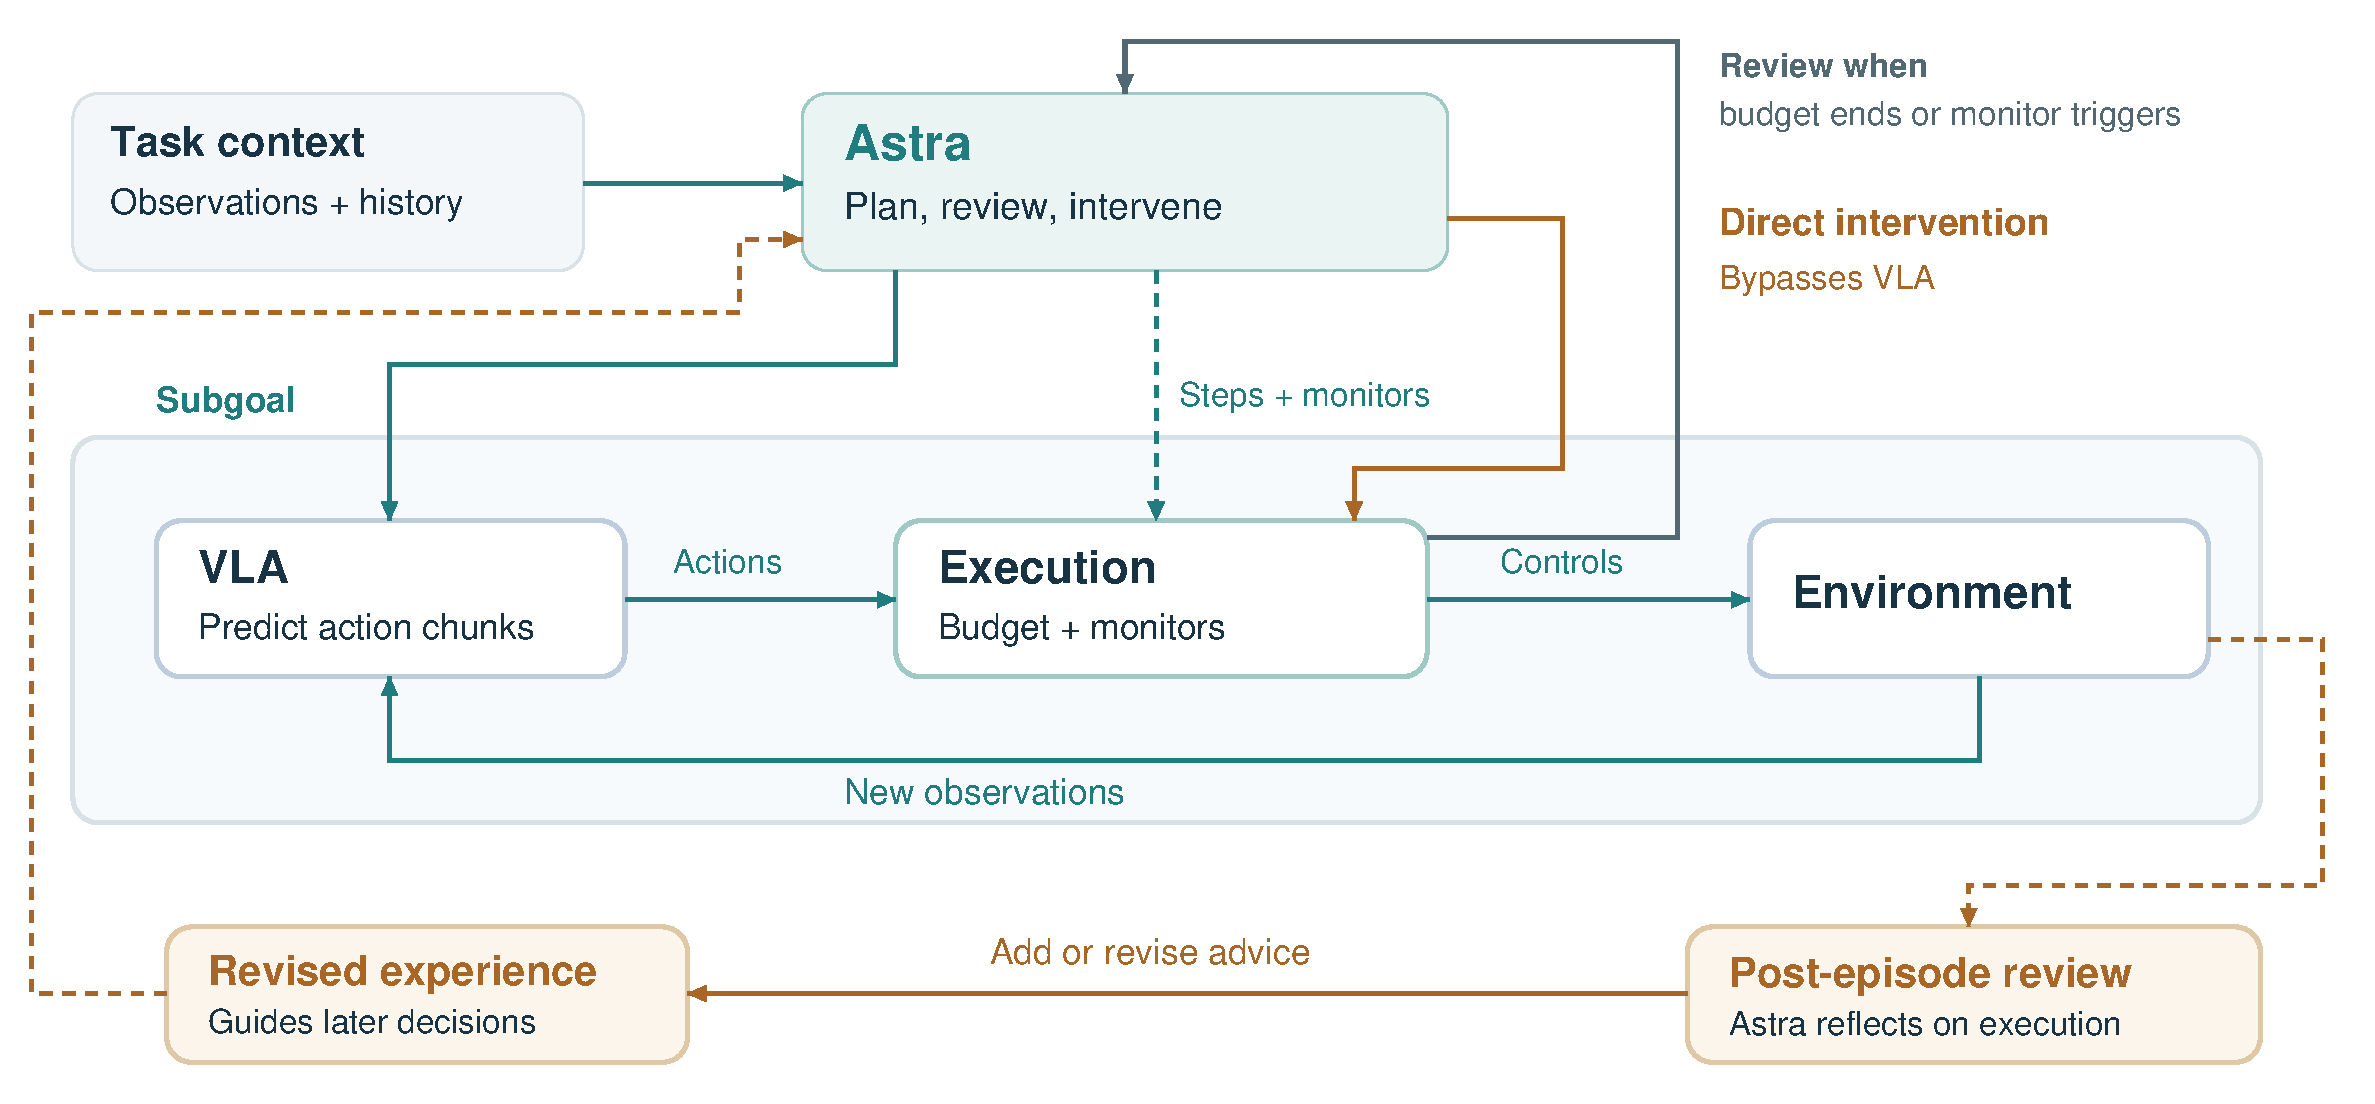
\includegraphics[width=\linewidth]{architecture.pdf}
\caption{Astra assigns execution budgets and selects monitors while the VLA responds to updated observations. Direct interventions bypass the VLA, and post-episode review revises experience for subsequent episodes.}
\label{fig:architecture}
\end{figure}

Astra can authorize a single action chunk, delegate multiple chunks before the next review, or directly issue end-effector targets in world coordinates and gripper commands. After a subgoal change or direct intervention, the VLA predicts a new action sequence using the latest observation and current subgoal before execution resumes.

History queries retrieve information no longer visible in the current observations, including reset demonstrations and intermediate frames. Astra initially samples frames from a requested interval, including its endpoints, and can narrow the interval or inspect individual frames when more detail is needed. Episode notes preserve task-relevant interpretations, unresolved hypotheses, and references to supporting frames. Global and task-specific experience remains available throughout the episode. All decisions rely on task instructions, RGB observations, and robot state available under standard RoboMME evaluation. The harness does not access privileged information such as ground-truth object states or oracle subgoals. Episode success is determined by official environment feedback.

\subsection{Grounded subgoals}

A grounded subgoal combines a RoboMME task template, semantic attributes, and target image points \citepending{robomme}. Astra identifies the relevant attributes from task history and the current scene. The harness then converts normalized image points into front-image pixel coordinates for the grounded instruction. For example, an InsertPeg grasp specifies which end of the peg to grasp and its image location:

\begin{quote}
\small\ttfamily\raggedright
pick up the peg by grasping the near end at <128, 64>
\end{quote}

The coordinates are illustrative. The insertion subgoal also specifies the left or right side of the box. The VLA receives the grounded instruction alongside the task instruction, current images, and robot state, following the representation used in its RoboMME training annotations. Applicable experience can guide target selection or recovery, while Astra determines whether the recorded conditions apply to the current scene. Experience can thus influence subgoal selection without changing the task requirements or the VLA's instruction vocabulary. Appendix~\ref{app:interfaces} provides conversion and validation details.

\subsection{Execution delegation and recovery}

To avoid unnecessary reviews during routine execution, Astra assigns a finite execution budget based on current observations, task history, and relevant experience. Initial budget recommendations are derived from subtask durations in the VLA training demonstrations, using the lower quartile of each subtask's duration distribution as a starting point. As experience accumulates, these recommendations are refined for specific task stages and execution difficulties.

For longer execution intervals, Astra can activate auxiliary monitors to detect events that may require attention. These include gripper-state changes, directional displacement beyond a specified threshold, and a lack of end-effector movement. When assigning a budget, Astra selects the relevant monitors, whose triggers prompt visual review before the budget expires. This allows longer periods of routine VLA execution without losing the ability to inspect potentially problematic events. Monitor thresholds and implementation details are provided in Appendix~\ref{app:configuration}.

The budget counts actual executed control steps rather than predicted actions. At chunk $j$, let $b_j$ denote the remaining budget and $h_j$ the number of predicted actions available for execution. We use the official GroundSG evaluation setting of 16 executed steps per action chunk as the maximum chunk length. The number of actions released is
\begin{equation}
 \ell_j=\min(16,h_j,b_j),\qquad b_{j+1}=b_j-u_j,
 \label{eq:budget}
\end{equation}
where $u_j\leq\ell_j$ is the number of actions actually executed. Execution may stop before all released actions are completed. As long as the budget remains and no monitor has triggered a review, the VLA predicts the next action chunk from updated observations. The VLA therefore continues to respond to changes in the scene without requiring Astra to review every chunk.

At each review during execution, Astra compares the latest observations with the intended subgoal and relevant history. It can extend execution, select a new subgoal, authorize one chunk at a time for closer supervision, or intervene directly. An incorrect target, for example, may require another history query and a revised subgoal, while a stalled contact motion may call for a local end-effector correction. After intervention, the VLA resumes from the resulting observation under Astra's next decision. Budgeted execution and event-triggered reviews allow the VLA to handle routine motion while Astra focuses on decisions and recovery.

\subsection{Cross-episode experience evolution}

The experience store records what Astra learns about task interpretation and VLA execution across episodes. Each entry contains an observation or recommendation, its applicable conditions, and references to supporting frames. Experience can guide target identification, execution budgets, monitor selection, and recovery. Existing entries can be revised when new evidence changes their recommendations or applicable conditions, with earlier versions preserved. New findings become available to subsequent episodes.

After each episode, Astra reviews the execution in the same agent session. The review draws on retained interactions and tool responses, episode notes, active experience, and official outcome and termination feedback. Astra can also inspect archived front and wrist images, starting with sparse samples and examining individual intervals in greater detail when needed. Execution records preserve selected budgets, executed steps, and review triggers. These records help Astra identify problematic stages and reconsider its earlier supervision and recovery decisions.

Based on this review, Astra adds new entries for findings not yet covered by the store and revises existing ones when new evidence changes their recommendations or applicable conditions. For example, hovering before a scheduled review may motivate a shorter budget for that stage or the use of a stationary-motion monitor. Experience from a temporal query may also be refined to distinguish tasks that refer to events before or after a particular observation. These updates turn individual outcomes into more specific guidance for future decisions.

Experience updates undergo structural and scope checks before being stored. During later episodes, Astra can refer to relevant entries when selecting subgoals, setting execution budgets, or choosing recovery actions. The resulting decisions can be traced back to the experience that informed them (Section~\ref{sec:results}). The harness thus adapts through accumulated and revised experience while keeping the VLA weights fixed.

% \section{Harness}
% \label{sec:harness}
% \subsection{System and task context}
% The harness connects Astra's task decisions to VLA execution and direct intervention (Figure~\ref{fig:architecture}). At each decision point, Astra receives the task instruction, current front and wrist RGB images, robot state, and a summary of the next action sequence predicted by the VLA. It can query archived observations and consult episode notes. Relevant global and task experience remains available throughout the episode. Forward kinematics is used to estimate the end-effector motion implied by the VLA's predicted joint actions. Episode success is determined by official environment feedback.

% \begin{figure}[!htbp]
% \centering
% 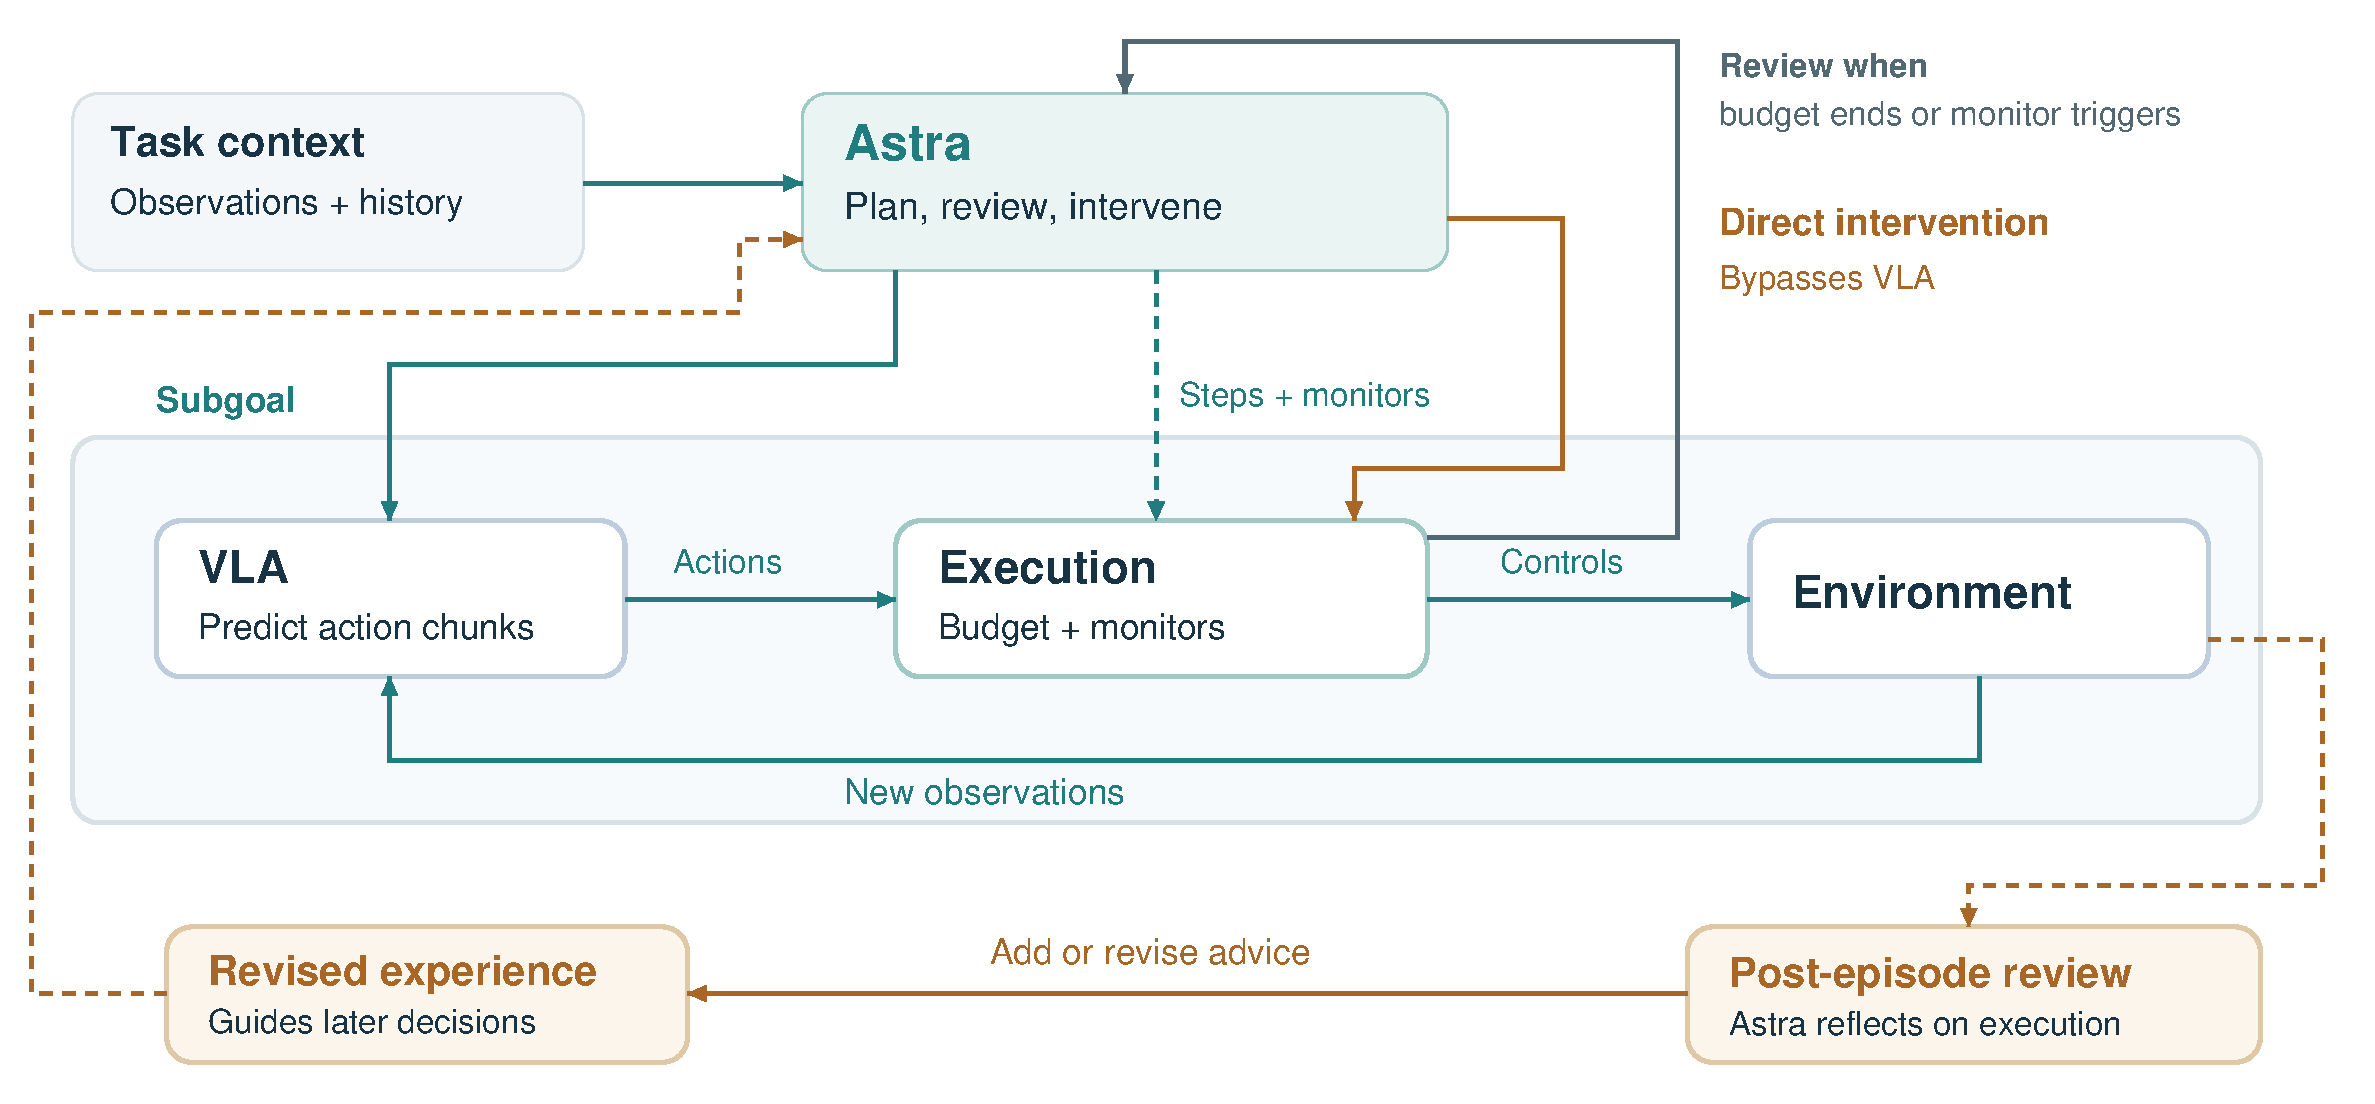
\includegraphics[width=\linewidth]{architecture.pdf}
% \caption{Astra sets execution budgets and selects monitors while the VLA reacts to new observations. Direct interventions bypass the VLA; post-episode review revises advice for later decisions.}
% \label{fig:architecture}
% \end{figure}

% The VLA uses the official RoboMME GroundSG checkpoint and maps its current observation and grounded subgoal to a joint-action sequence. Astra can permit one action chunk, let the VLA execute several chunks before review, or directly specify end-effector targets in world coordinates and gripper commands. Direct intervention bypasses the VLA but acts on the same robot and episode. After a subgoal change or direct intervention, the VLA predicts a new action sequence from the latest observation and current subgoal before execution resumes.

% History queries recover evidence absent from the current views, including reset demonstrations and intermediate observations. Astra first samples a requested interval, including its endpoints, then narrows the interval or inspects original frames when necessary. Episode notes retain task-relevant interpretations and unresolved hypotheses with frame references, allowing Astra to revisit their supporting observations when needed. The agent uses task instructions, front and wrist images, and robot state available under standard RoboMME evaluation. It receives no privileged environment information such as ground-truth object states or oracle subgoals.

% \subsection{Grounded subgoals}
% A grounded subgoal combines a RoboMME task template, semantic attributes, and target image points \citepending{robomme}. Astra resolves the attributes from history and the current scene; the harness converts normalized points to front-image pixel coordinates and inserts them into the instruction. For example, an InsertPeg grasp specifies the near or far end of the peg and its image location:
% \begin{quote}
% \small\ttfamily\raggedright pick up the peg by grasping the near end at <128, 64>
% \end{quote}
% The coordinates here are illustrative image references. Insertion additionally specifies the left or right side of the box. The VLA receives this grounded instruction with the task instruction, current images, and robot state, matching the representation used in its RoboMME training annotations. Applicable experience can advise target selection or recovery, while Astra judges whether its conditions fit the scene. Experience can therefore influence which subgoal is selected without changing the task requirements or the controller's instruction vocabulary. Appendix~\ref{app:interfaces} gives conversion and validation details.

% \subsection{Execution delegation and recovery}
% To avoid unnecessary reviews during routine execution, Astra assigns a finite execution budget based on current observations, task history, and relevant experience. Initial budget advice comes from the number of control steps used to complete subtasks in training demonstrations; the lower quartile of each subtask's duration distribution provides a starting point. Subsequent experience refines these recommendations for particular stages and observed execution difficulties.

% Longer execution intervals can be paired with auxiliary monitoring tools. Gripper-state changes, directional displacement beyond a specified threshold, or a lack of end-effector movement can indicate a stage transition or potential execution problem. Astra selects the relevant monitors when assigning a budget. A detected condition prompts visual review, allowing Astra to inspect progress before the full interval ends. These tools let Astra retain longer budgets during routine motion while watching for events that may require attention. Thresholds and implementation details appear in Appendix~\ref{app:configuration}.

% The budget counts actual executed control steps. At chunk $j$, let $b_j$ be the remaining budget and $h_j$ the number of predicted actions available for execution. Execution uses
% \begin{equation}
%  \ell_j=\min(16,h_j,b_j),\qquad b_{j+1}=b_j-u_j,
%  \label{eq:budget}
% \end{equation}
% where $\ell_j$ is the number of actions released for execution and $u_j\leq\ell_j$ is the number actually executed, which may be smaller if execution stops early. After executing these steps, the VLA predicts the next action chunk from the latest observations. Thus the controller continues to respond to the scene while Astra reviews at the selected interval or when a monitor triggers.

% At a nonterminal review with a valid execution state, Astra compares the new observations with the intended subgoal and relevant history. It can extend execution, choose another subgoal, permit one chunk at a time for close supervision, or intervene directly. For example, an incorrect target may call for another history query and a revised subgoal, whereas a stalled contact motion may call for a local end-effector correction. After intervention, the VLA receives the resulting observation and resumes control under Astra's next decision. Budgeted execution and event-triggered review therefore support both sustained VLA operation and targeted recovery.

% \subsection{Cross-episode experience evolution}
% The experience store captures what Astra learns about task interpretation and VLA execution across episodes. Entries pair an observation or recommendation with its applicable conditions and supporting frames. Advice can concern target identification, review intervals, monitoring choices, or recovery. Revisions replace outdated recommendations while preserving their earlier versions. Each episode uses the available global and task-specific experience, and new findings become available to subsequent episodes.

% After the episode ends, Astra performs the review in the same agent session. Its inputs include retained interactions and tool responses, episode notes, active experience, and the official outcome and termination status. It can query archived front and wrist images, moving from sparse sampling to closer inspection. Execution records include the selected budgets, the number of steps executed, and the conditions that prompted review. Astra uses these records to identify problematic stages, assess its earlier supervision and recovery decisions, and determine whether the findings should update existing experience.

% Astra adds an entry when review identifies a transferable finding, or revises an existing entry when new evidence changes its recommendation or applicable conditions. Findings already covered by the store require no update. For example, hovering observed before a scheduled review can motivate a shorter budget for that phase or the use of a stationary-motion monitor. A recommendation that works for one temporal query can be revised to distinguish before-event and after-event tasks. In this way, experience develops from individual outcomes into conditional guidance for later decisions.

% Updates pass structural and scope checks before entering the experience store. Later decisions can cite the relevant entries when choosing a subgoal, review interval, or recovery action, making it possible to trace how past outcomes informed subsequent actions (Section~\ref{sec:results}). Adaptation takes place through this evolving context while the VLA weights remain fixed.
